%%%%%%%%%%%%%%%%%%%%%%%%%%%%%
%% Styles, packages and new commands
\input{../../Main/ML_Main.tex}
%%%%%%%%%%%%%%%%%%%%%%%%%%%%%
%% Edit the title page
\title{Machine Learning}
\subtitle{Module 8.1 - Unsupervised Learning: clustering}
\author[MOB]{Marc-Olivier Boldi}
\institute[HEC MSc Mgt BA]{Master in Management, Business Analytics, HEC UNIL}
\date{Spring 2025}
%%%%%%%%%%%%%%%%%%%%%%%%%%%%%
%%%%%%%%%%%%%%%%%%%%%%%%%%%%%
%%%%%%%%%%%%%%%%%%%%%%%%%%%%%
%%%%%%%%%%%%%%%%%%%%%%%%%%%%%
\begin{document}
%%%%%%%%%%%%%%%%%%%%%%%%%%%%%
\begin{frame}
  \titlepage
\end{frame}
%%%%%%%%%%%%%%%%%%%%%%%%%%%%%
\begin{frame}
\frametitle{Table of Contents}
	\tableofcontents
\end{frame}
%%%%%%%%%%%%%%%%%%%%%%%%%%%%%
\section{Concepts}
%%%%%%%%%%%%%%%%%%%%%%%%%%%%%
\begin{frame}
\frametitle{Clusters}
A {\bf cluster} is a group of instances that share some common characteristics measured by the features. They are {\bf similar}. \\ 
\vspace{0.3cm}
Unlike classification (supervised learning) where groups are already defined, clustering aims at finding groups that {\bf do not exist a priori}.
\end{frame}
%%%%%%%%%%%%%%%%%%%%%%%%%%%%%
\begin{frame}
\frametitle{Hierarchical clustering and partitioning}
Two different approaches: 
\begin{itemize} 
\item Hierarchical clustering: methods based on a {\bf dissimilarity matrix} (hierarchical clustering).
\item Partitioning: methods based on the value of the features (K-Means, PAM). 
\end{itemize}
\end{frame}
%%%%%%%%%%%%%%%%%%%%%%%%%%%%%
\section{Hierarchical clustering}
%%%%%%%%%%%%%%%%%%%%%%%%%%%%%
\begin{frame}
\frametitle{Concept}
Hierarchical clustering algorithms
\begin{itemize}
\item Take a {\bf dissimilarity matrix} as input: the features are used to compute dissimilarities between instances. The feature values are not by the algorithm strickly speaking.  
\item Can be of two types: {\bf agglomerative} (e.g., AGNES) or {\bf divisive} (not treated). 
\end{itemize}
In agglomerative algorithm, once two instances are clustered, they cannot be separated.
\end{frame}
%%%%%%%%%%%%%%%%%%%%%%%%%%%%%
\begin{frame}
\frametitle{AGNES}
Accronym for {\bf AGglomerative NESting}: a sequential algorithm: 
\begin{enumerate}
\item To start each instance is a cluster in itself. 
\item Merge the two closest clusters into one bigger cluster.
\item Repeat 2 until only one cluster remains.
\end{enumerate}
To merge two clusters (2), we need a {\bf linkage method}. To link two clusters, we need {\bf dissimilarities}.
\end{frame}
%%%%%%%%%%%%%%%%%%%%%%%%%%%%%
\begin{frame}
\frametitle{Dissimilarity}
A {\bf dissimilarity} between two instances with features $x$ and $x'$ is a function $d(\cdot, \cdot)$ such that
\begin{itemize}
\item Non-negativity: $d(x,x')\geq 0$,
\item Nullity: $d(x,x') = 0$ iff $x=x'$,
\item Symmetry: $d(x,x') = d(x',x)$,
\end{itemize}
If further it satisfies the triangle inequality, 
$$
d(x, x') + d(x', x'') \geq d(x, x''),
$$
then it is called a {\bf distance}
\end{frame}
%%%%%%%%%%%%%%%%%%%%%%%%%%%%%
\begin{frame}
\frametitle{For numerical features}
A general distance: {\bf Minkowski}, $q \geq 1$
$$
d(x,x') = \left(\sum_{j=1}^p |x_j - x'_j|^q\right)^{1/q}
$$
\scriptsize
Special cases:
\begin{itemize}
\item {\bf Euclidean} for $q=2$ (the most used),
$$
d(x,x') = \sqrt{\sum_{j=1}^p (x_{j} - x'_{j})^2}
$$
\item {\bf Manhattan} for $q=1$, 
$$
d(x,x') = \sum_{j=1}^p \vert x_j - x'_j \vert
$$
\item {\bf Maximum distance} $q=\infty$, 
$$
d(x,x') = \max_{j=1,\ldots p} \vert x_j - x'_j\vert
$$
\end{itemize}
\normalsize
\end{frame}
%%%%%%%%%%%%%%%%%%%%%%%%%%%%%
\begin{frame}[fragile]
\frametitle{Numerical features}
Example on the {\tt iris} data. The Euclidean distance between instances 1 and 2 is $0.54$\\
\scriptsize
\begin{verbatim}
> iris[1:2,-5]
  Sepal.Length Sepal.Width Petal.Length Petal.Width 
1          5.1         3.5          1.4         0.2 
2          4.9         3.0          1.4         0.2 
> dist(iris[1:2, -5], p=2)
  0.5385165
\end{verbatim}
\normalsize
In detail,
$$
\sqrt{(5.1-4.9)^2+(3.5-3.0)^2+(1.4-1.4)^2+(0.2-0.2)^2}=0.54
$$
\end{frame}
%%%%%%%%%%%%%%%%%%%%%%%%%%%%%
\begin{frame}
\frametitle{Categorical and mixed features types}
When categorical features are present in the data set, the {\bf Gower index} can be used. It combines dissimilarities to build a global one: 
$$
d_{ij} = \frac{\sum_{k=1}^p w_k d_{ij,k}}{\sum_{k=1}^p w_k}
$$ 
is the dissimilarity between instances $i$ and $j$ over the $p$ features.\\
\vspace{0.2cm}
The weight $w_k$ are always 1, except if $x_{ik}$ or $x_{jk}$ is missing, in which case it is $0$. The dissimilarity $d_{ij,k}$ depends on the type of the feature $x_k$:
\begin{itemize}
\item Numerical: 
$$
d_{ij,k} = |x_{ik} - x_{jk}|/r_k,
$$
where $r_k$ is the range of variable $k$ (i.e., max $-$ min),
\item Categorical: $d_{ij,k} = 1$ if $x_{ik}\neq x_{jk}$, $d_{ij,k} = 0$ if $x_{ik}= x_{jk}$.
\end{itemize}
\end{frame}
%%%%%%%%%%%%%%%%%%%%%%%%%%%%%
\begin{frame}[fragile]
\frametitle{Mixed features types}
Example:
\scriptsize
\begin{verbatim}
  Sepal.Length Sepal.Width Petal.Length Petal.Width    Color    Species
1          5.1         3.5          1.4         0.2    mauve     setosa
2          4.9         3.0          1.4         0.2   violet     setosa
3          4.7         3.2          1.3         0.2   violet  virginica
\end{verbatim}
\normalsize
The ranges are respectively $3.6,2.4,5.9,2.4$ (computed on the whole data set). Then,
\scriptsize
\begin{eqnarray*}
d_{12} &=& \frac{1}{6}\left(\frac{|5.1-4.9|}{3.6} + \frac{|3.5-3.0|}{2.4} + \frac{|1.4-1.4|}{5.9} + \frac{|0.2-0.2|}{2.4} + 1 + 0\right) = 0.2106.\\
\\
d_{13} &=& 0.3755\\
\\
d_{23} &=& 0.1926
\end{eqnarray*}
\end{frame}
%%%%%%%%%%%%%%%%%%%%%%%%%%%%%
\begin{frame}
\frametitle{Linkage}
Once the matrix of dissimilarities between all the instances is computed, we use {\bf linkage} to merge the two clusters:
\small
\begin{itemize}
\item {\bf Single linkage}: For all pairs of clusters $A$ and $B$, compute the smallest dissimilarity between each pair of cluster members,
$$
d(A,B) = \min \{d(x,x'): x\in A,\; x' \in B\}
$$
Link $A$ and $B$ with the smallest $d(A,B)$.
\item {\bf Complete linkage}: For all pairs of clusters $A$ and $B$, compute the largest dissimilarity between each pair of cluster members,
$$
d(A,B) = \max \{d(x, x'): x\in A,\; x' \in B\}
$$
Link $A$ and $B$ with the smallest $d(A,B)$.
\item {\bf Ward}'s method: merges the two clusters $A$ and $B$ such that, after the merging, the total within variance is minimum\footnote{Other criteria are possible. Several algorithms exists (e.g., Ward 1963, Murtagh and Legendre 2014).}.
\end{itemize}
\normalsize
\end{frame}
%%%%%%%%%%%%%%%%%%%%%%%%%%%%%
\begin{frame}
\frametitle{Dendrogram}
The {\bf dendrogram} is a graphical representation of the hierarchical clustering. It shows
which clusters are grouped at each step $k$, together with the dissimilarity on the $y$-axis ate which they have been clustered.
\end{frame}
%%%%%%%%%%%%%%%%%%%%%%%%%%%%%%%
\begin{frame}
\frametitle{Example}
Italian cities: Bari, Firenze, Napoli, Roma, Torino.
\begin{center}
\begin{columns}
\begin{column}{0.6\textwidth}
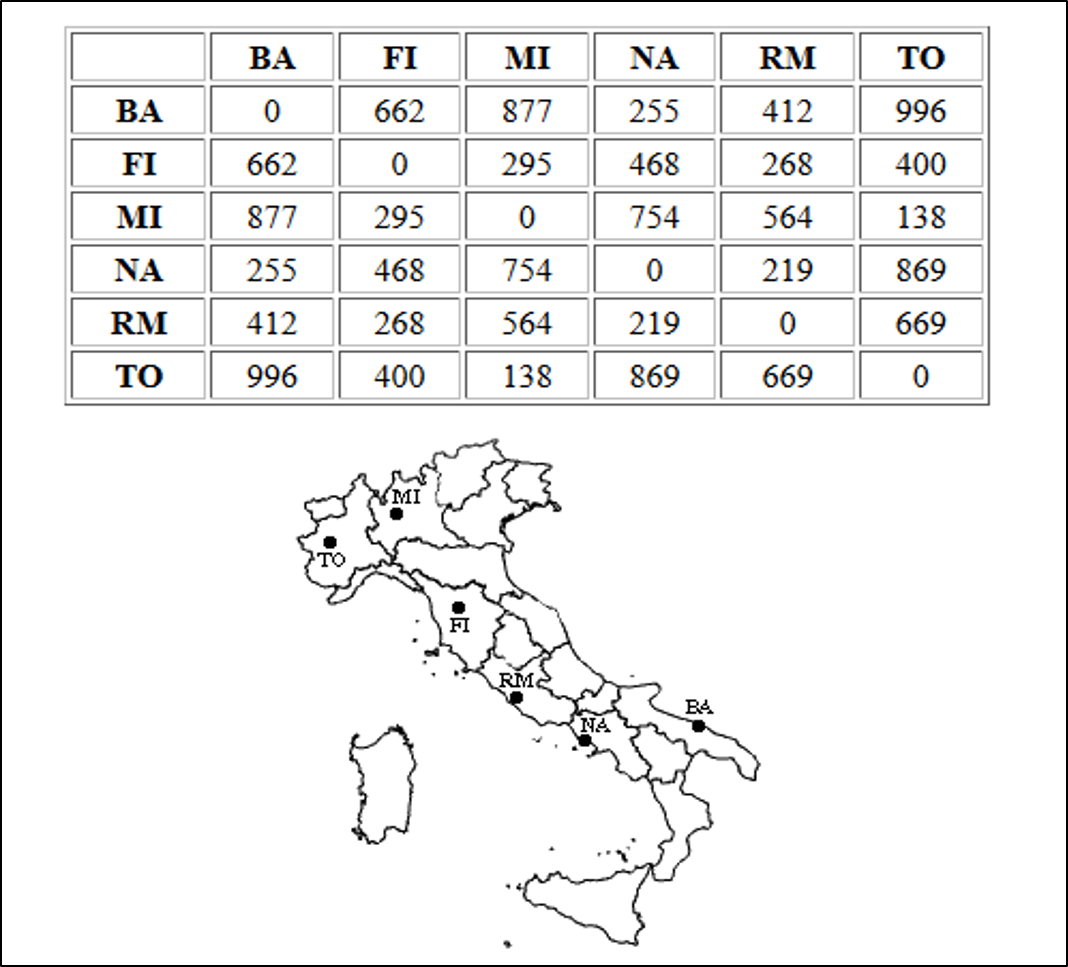
\includegraphics[width=6cm]{../../Graphs/Italy1.png}
\end{column}
\begin{column}{0.4\textwidth}
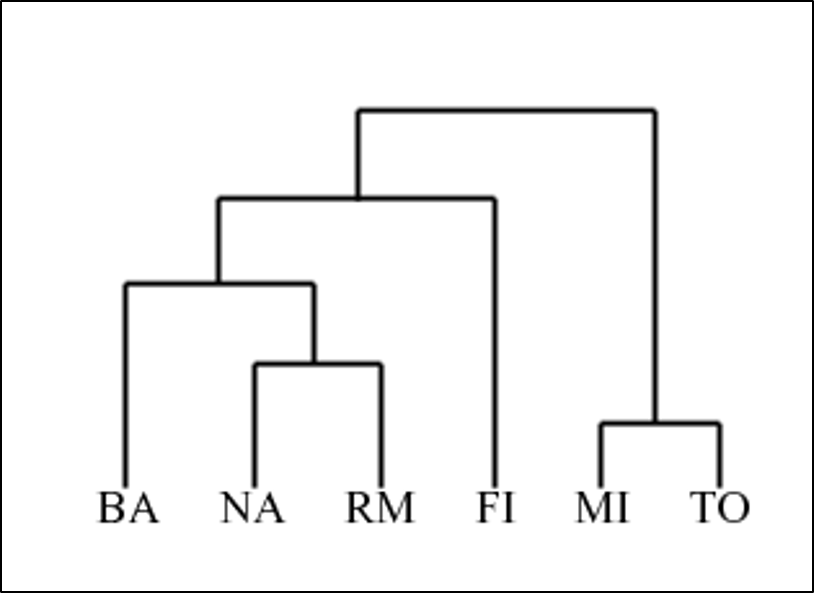
\includegraphics[width=4cm]{../../Graphs/Italy2.png}
\end{column}
\end{columns}
\end{center}
\tiny
Source: \url{https://home.deib.polimi.it/matteucc/Clustering/tutorial_html/hierarchical.html}
\normalsize
\end{frame}
%%%%%%%%%%%%%%%%%%%%%%%%%%%%%
\begin{frame}
\frametitle{Divisive hierarchical clustering}
AGNES is {\bf agglomerating} because it starts from individual points and run up to a unique cluster, merging clusters one after the other. \\
\vspace{0.3cm}
It is called "hierarchical" because when an instance is attached to a group, it cannot be separated from it anymore.\\
\vspace{0.3cm} 
There also exists {\bf divisive} hierarchical clustering, {\bf DIANA}, for DIvise ANAlysis. It starts from one unique cluster with all the instances, and splits clusters one after the other, going down to one instance per cluster. \\
\vspace{0.3cm} 
Divise clustering is seen as more complex than agglomerative because, at each step, there exist a lot of possibilities to split one cluster into two, whereas there is only one way to merge two clusters into one.
\end{frame}
%%%%%%%%%%%%%%%%%%%%%%%%%%%%%
%%%%%%%%%%%%%%%%%%%%%%%%%%%%%
\section{Partitioning methods}
%%%%%%%%%%%%%%%%%%%%%%%%%%%%%
%%%%%%%%%%%%%%%%%%%%%%%%%%%%%
\begin{frame}
\frametitle{Partitioning methods}
Unlike the hierarchical clustering, {\bf partitioning methods} apply for a given number of clusters. \\
\vspace{0.3cm}
Starting from an initial assignment of instances to $k$ clusters, the method allocates the instances to clusters such that a given criterion is optimized. \\
\vspace{0.3cm}
Two popular methods are 
\begin{itemize}
\item The {\bf K-means}.
\item The {\bf Partitioning Around the Medoid} (PAM). 
\end{itemize}
\end{frame}
%%%%%%%%%%%%%%%%%%%%%%%%%%%%%
\begin{frame}
\frametitle{K-means}
For $k$ clusters:
\begin{enumerate}
\item The initial clustering is random: assign each instance to one cluster at random.
\item Compute the centers of the clusters. 
\item Each instance is then re-assigned to the cluster with the closest center.
\item Step 2. and 3. are repeated until a convergence criterion is satisfied.
\end{enumerate}
The K-means is suitable for {\bf numerical features only}. The Euclidean distance is often used.
\end{frame}
%%%%%%%%%%%%%%%%%%%%%%%%%%%%%
\begin{frame}
\frametitle{K-means}
Illustration on simulated data, with $k=2$. Below, the data ($p=2$)
\begin{center}
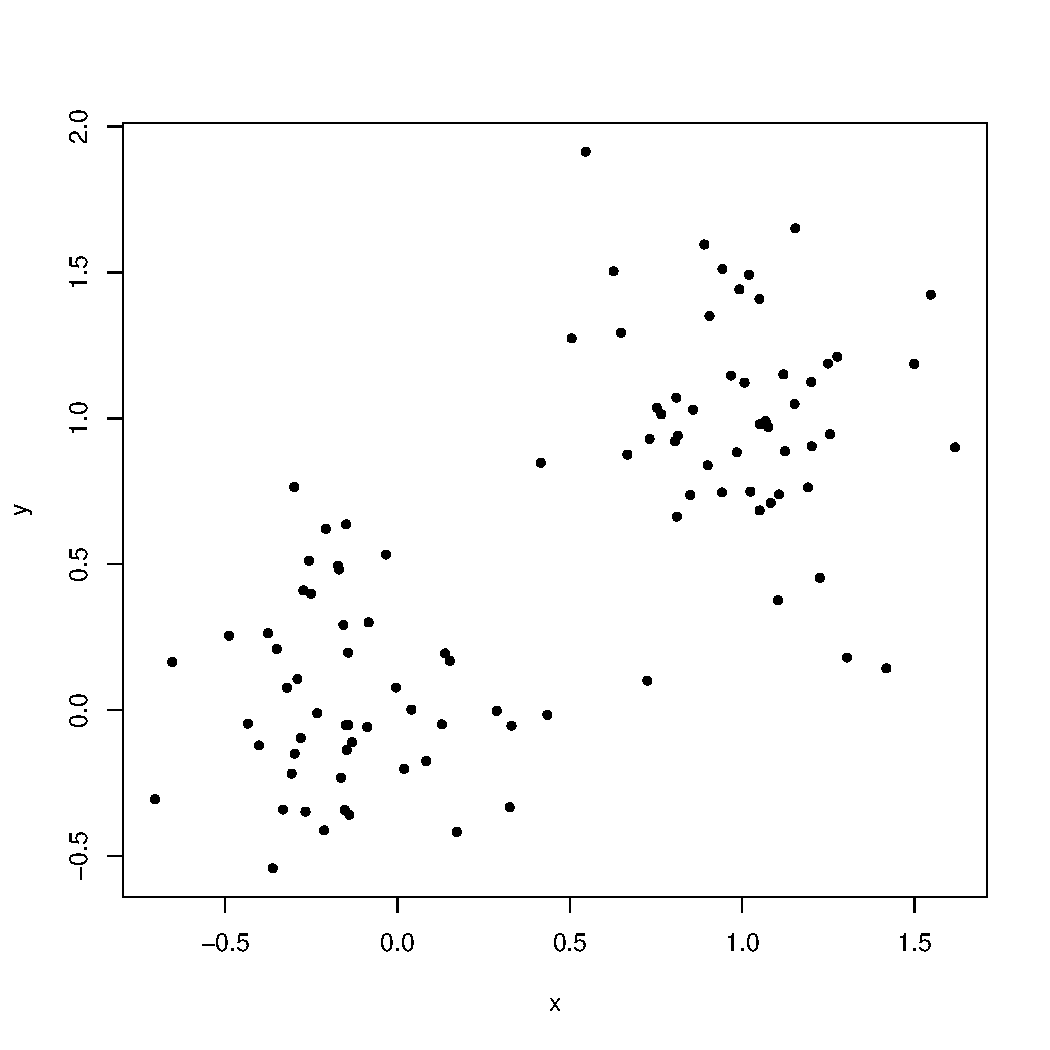
\includegraphics[width=7cm]{../../Graphs/kmeans1.pdf}
\end{center}
\end{frame}
%%%%%%%%%%%%%%%%%%%%%%%%%%%%%
\begin{frame}
\frametitle{K-means}
First step, each instance is randomly assigned (circles and triangles). The centers are computed (dots).
\begin{center}
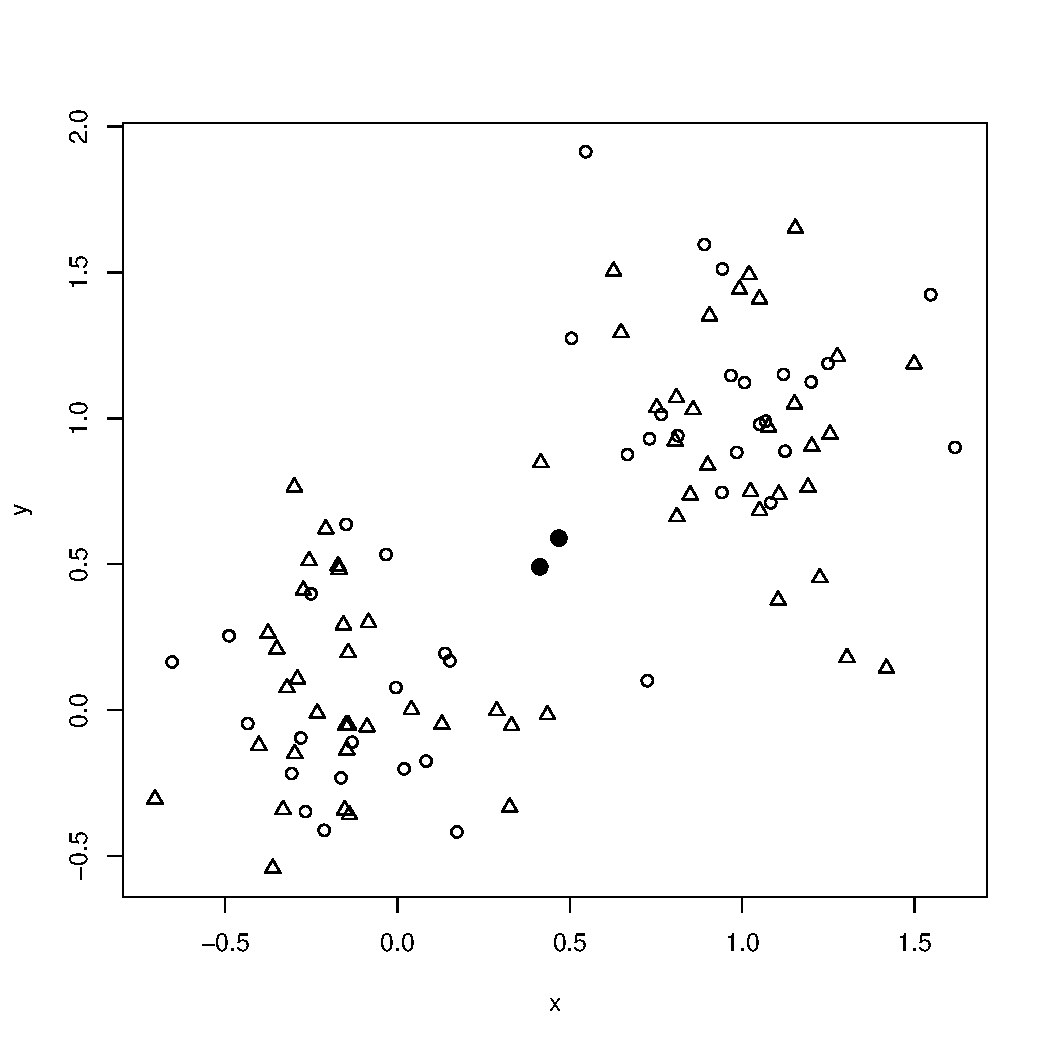
\includegraphics[width=7cm]{../../Graphs/kmeans2.pdf}
\end{center}
\end{frame}
%%%%%%%%%%%%%%%%%%%%%%
\begin{frame}
\frametitle{K-means}
Next step, instances are re-assigned to the closest center. Then, new centers are computed. The clustering is already finished.
\begin{center}
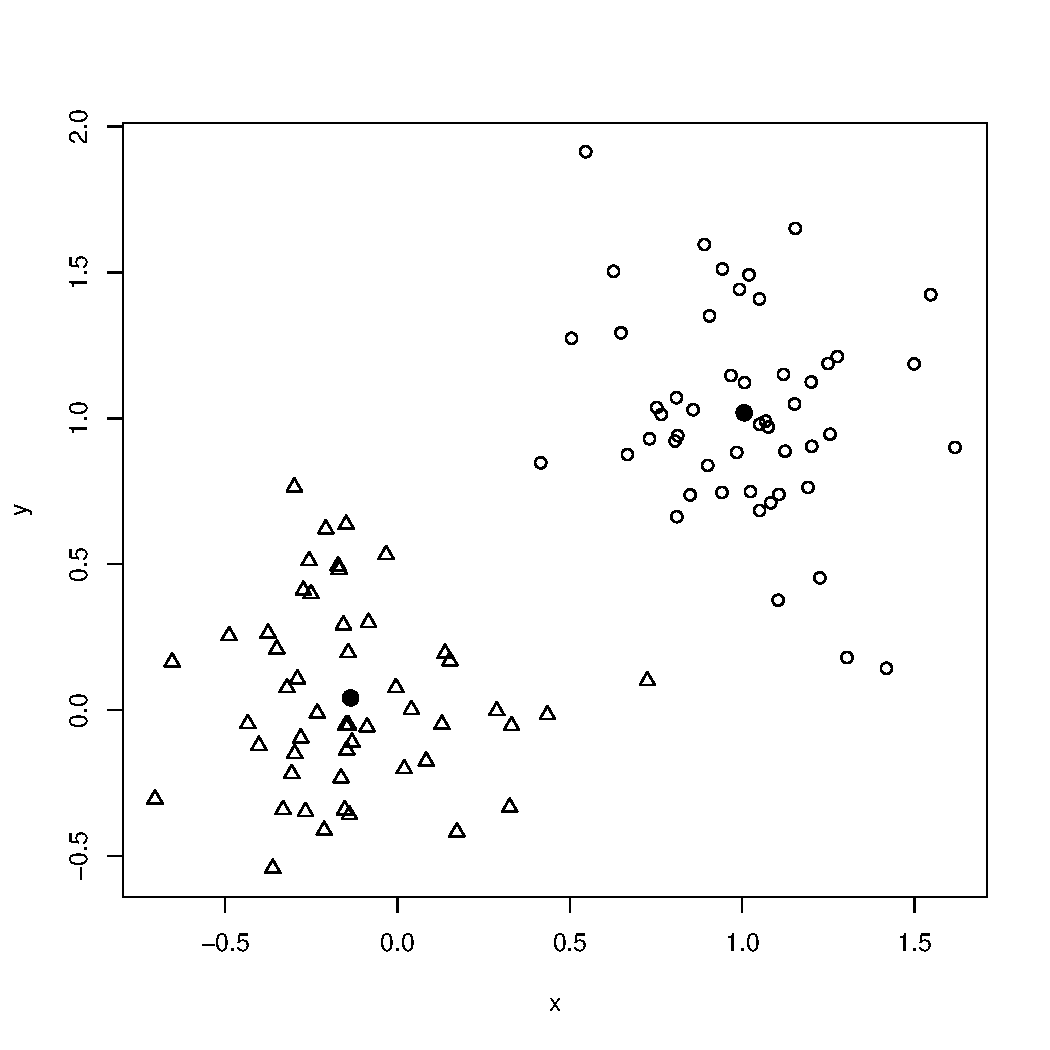
\includegraphics[width=7cm]{../../Graphs/kmeans3.pdf}
\end{center}
\end{frame}
%%%%%%%%%%%%%%%%%%%%%%
\begin{frame}
\frametitle{K-means}
Illustration for $k=3$ clusters.
\begin{center}
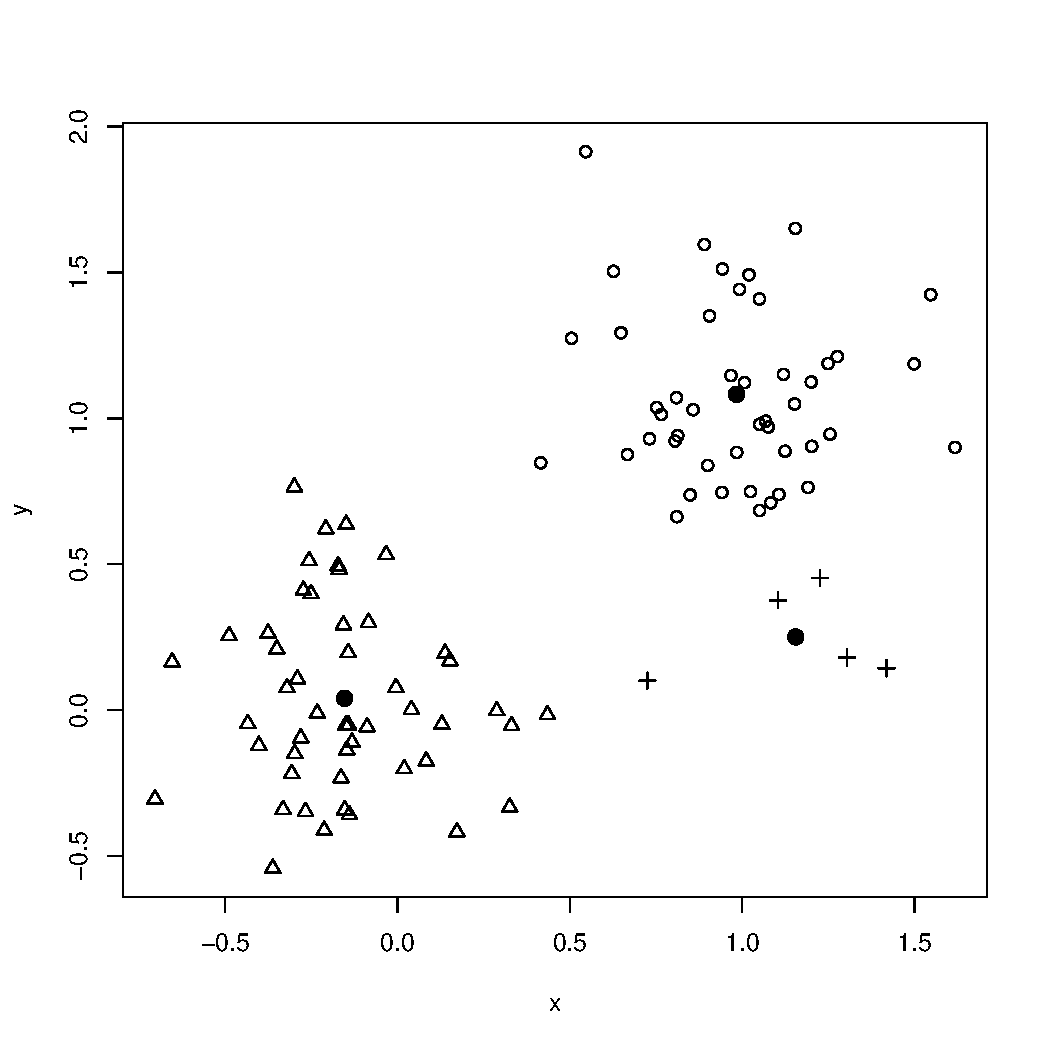
\includegraphics[width=7cm]{../../Graphs/kmeans4.pdf}
\end{center}
\end{frame}
%%%%%%%%%%%%%%%%%%%%%%%
\begin{frame}
\frametitle{Partitioning Around the Medoid}
{\bf PAM} extends the K-mean to {\bf features of mixed types} (numerical and categorical) by extending the definition of the center of the cluster to {\bf a medoid}.\\
\vspace{0.3cm} 
The medoid of cluster is the most representative instance belonging to it.\\
\vspace{0.3cm}
The medoid of a cluster $A$ is the instance with smallest sum of dissimilarities with the other instances in the cluster $A$:
$$
m_A = \arg \min_{x \in A} \sum_{y\in A; y\neq x} d_{xy}
$$
Unlike for the K-means, where the center is computed by averaging the features values (and thus may not be an instance of the data base), the medoid is an instance of its cluster.\\ 
\vspace{0.3cm}
Therefore, PAM can be used for both {\it numerical and categorical features}.
\end{frame}
%%%%%%%%%%%%%%%%%%%%%%%
\begin{frame}
\frametitle{Example}
With the Italian cities, consider the cluster \{BA, NA, RM\}. Then the medo{\"\i}d is NA. Indeed, the sum of dissimilarities are
\begin{itemize}
\item BA: $d_{BA,NA}+d_{BA,RM} = 255+412=667$
\item NA: $d_{NA,BA}+d_{NA,RM} = 255+219=474$
\item RM: $d_{RM,BA}+d_{RM,NA} = 212+219=631$
\end{itemize}
Thus NA is the most representative city of this cluster. \\
\vspace{0.3cm}
Note that the medo{\"\i}d of cluster \{MI, TO\} is either MI or TO (at random). 
\end{frame}
%%%%%%%%%%%%%%%%%%%%%%%
\section{Number of clusters}
%%%%%%%%%%%%%%%%%%%%%%%
\begin{frame}
\frametitle{Choice or selection?}
The number of clusters is often an {\bf arbitrary choice} guided by the domain and the business application. This approach should be preferred if possible.\\
\vspace{0.3cm}
It is also possible to select of the number of clusters with an index. There are a lot of such index\footnote{There are 30 index available in the function {\tt NbClust} in {\tt R}.}.\\
\vspace{0.3cm}
In this course, we see
\begin{itemize}
\item The {\bf total within-cluster sum of squares} (TWSS),
\item The {\bf silhouette}.
\end{itemize}
In practice, the index is computed for a clustering with $1$, $2$, $3$, etc., clusters and the best choice is made.
\end{frame}
%%%%%%%%%%%%%%%%%%%%%%%%%%%%%
\begin{frame}
\frametitle{Total within-cluster sum of squares}
The sum of squares within cluster $C$, whose center (mean or medoid) is $x_C$, is the  
$$
\quad W_C=\sum_{i \in C} \Vert x_i - x_C\Vert^2 = \sum_{i \in C}\sum_{j=1}^p (x_{ij} - x_{Cj})^2.
$$
The TWSS is the sum of all $W_k$ over the $K$ clusters $C_1,\ldots,C_K$,
$$
\sum_{k=1}^K W_{C_k}
$$
The Each time a cluster is created ($K \rightarrow K+1$), TWSS diminishes. The number of clusters is selected at {\bf an elbow} on the graph.
%\item The {\bf Gap} statistics:
%$$
%G_n(k) = E_{k,n}^* - \log(W_k)
%$$
%where $E^*_{k,n}$ is the expected value of $\log(W_k)$ under a reference distribution, computed by bootstrapping. The larger $G_n(k)$, the better the clustering.
\end{frame}
%%%%%%%%%%%%%%%%%%%%%%%%%%%%%
\begin{frame}
\frametitle{Example}
Clustering on data with TWSS (dendrogram with complete linkage):
\begin{center}
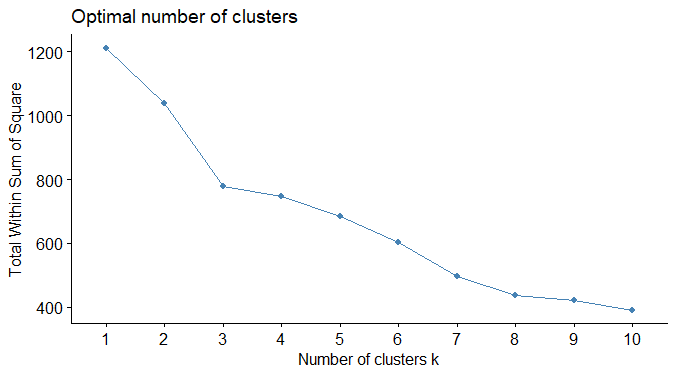
\includegraphics[width=8cm]{../../Graphs/Nb_agnes_hc_wss.png}
\end{center}
$k=3$ is a good choice here.
\end{frame}
%%%%%%%%%%%%%%%%%%%%%%%%%%%%%
\begin{frame}
\frametitle{Silhouette}
The {\bf silhouette} measures how "well" an instance is within its cluster. \\
\vspace{0.3cm}
Consider an instance $x$ assigned to cluster $C$. Let $d(x,A)$ be {\bf the dissimilarity from $x$ to any cluster $A$}: the average dissimilarity between $x$ and all the instances in cluster $A$:
$$
d(x,A) = \frac{1}{|A|} \sum_{y\in A} d_{xy}.
$$ 
In particular, {\bf $d(x, C)$ is the dissimilarity from $x$ to its cluster}.\\
\vspace{0.3cm}
A small $d(x,C)$ indicates a good clustering of $x$ within its cluster $C$.
\end{frame}
%%%%%%%%%%%%%%%%%%%%%%%
\begin{frame}
\frametitle{Silhouette}
Now, consider $d(x,\bar{C})$, the smallest average dissimilarities from $x$ to all the clusters to which it is not assigned (all but $C$):
$$
d(x,\bar{C}) = \min_{A\neq C} d(x, A) 
$$
This measures how $x$ is separated from the other clusters.\\
\vspace{0.3cm} 
A large $d(x,\bar{C})$ indicates a good separation of $x$ from all the other clusters (i.e., the ones in which $x$ is not).
\end{frame}
%%%%%%%%%%%%%%%%%%%%%%%%%
\begin{frame}
\frametitle{Silhouette}
The silhouette of $x$ combines 
\begin{itemize}
\item $d(x, C)$, how well $x$ is integrated to its cluster $C$, and 
\item $d(x,\bar{C})$, how well $x$ is separated from the other clusters.
\end{itemize}
The silhouette of $x$ is
$$
s_x=\frac{d(x,\bar{C})-d(x,C)}{\max\left\{d(x,\bar{C}),d(x,C)\right\}}
$$
The denominator ensures that $-1\leq s_x\leq 1$. \\
\vspace{0.3cm}
The larger $s_x$, the better the clustering of $x$ in $C$.
\end{frame}
%%%%%%%%%%%%%%%%%%%%%%%
\begin{frame}
\frametitle{Average silhouette}
The {\bf average silhouette} of all instances is taken as a measure of the {\bf goodness of the clustering}:
$$
s = \frac{1}{n}\sum_{i=1}^n s_{x_i}.
$$
The larger the average silhouette $s$, the better the clustering overall. The number of clusters $k$ should maximize the average silhouette.\\
\vspace{0.3cm}
The average silhouette should not be interpreted for itself. 
\end{frame}
%%%%%%%%%%%%%%%%%%%%%%%%%
\begin{frame}
\frametitle{Example}
Clustering on data with average silhouette:
\begin{center}
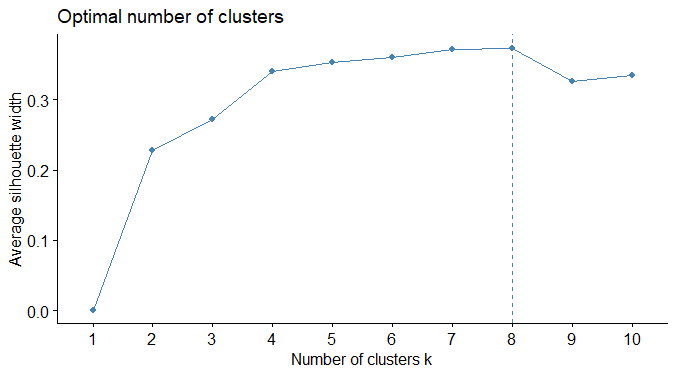
\includegraphics[width=8cm]{../../Graphs/Nb_pam_sil.png}
\end{center}
$k=8$ is a good choice here.
\end{frame}
%%%%%%%%%%%%%%%%%%%%%%%%%
\begin{frame}
\frametitle{Silhouette plot}
A detailed analysis of the clustering can be obtained using the {\bf silhouette plot} shows: the silhouettes of all the instances.
\begin{center}
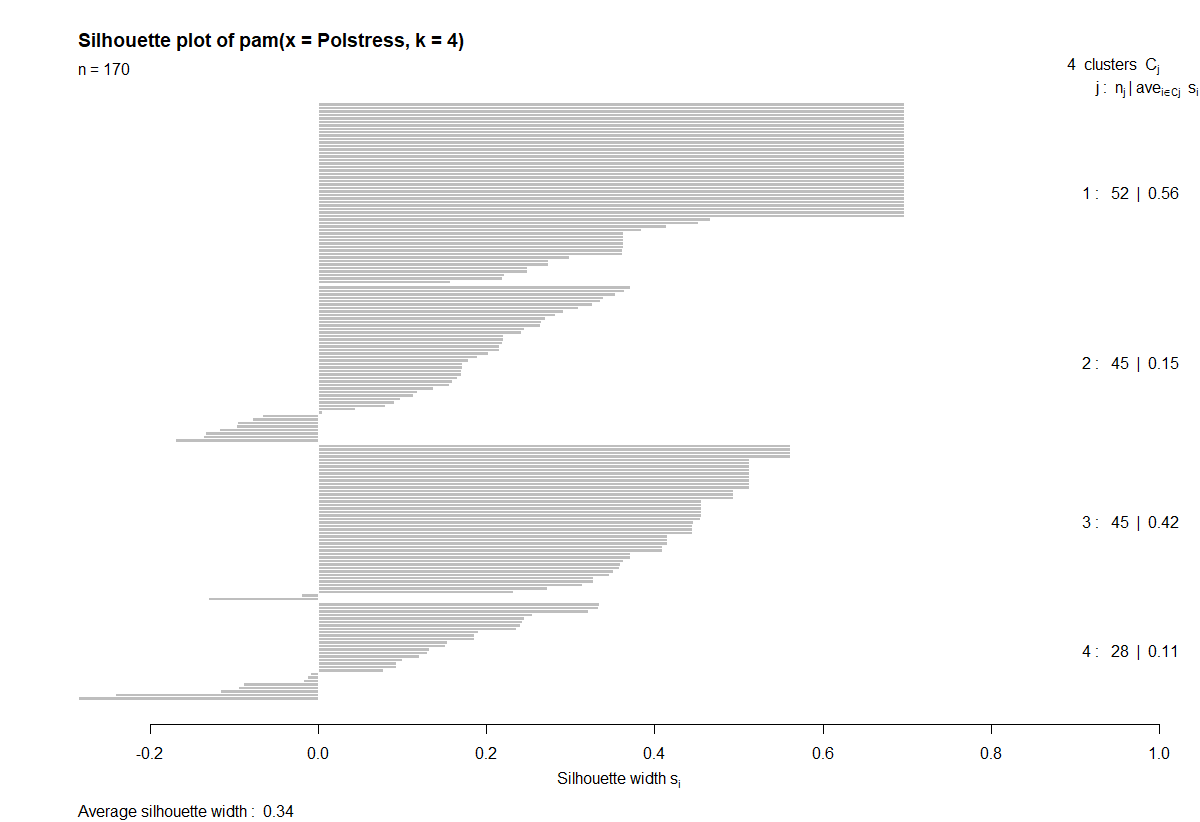
\includegraphics[width=8cm]{../../Graphs/Polstress-silhou.png}
\end{center}
Clusters 1 and 3 are well formed, Clusters 2 and 3 are less homogeneous. 
\end{frame}
%%%%%%%%%%%%%%%%%%%%%%%%%
\begin{frame}
\frametitle{Silhouette plot}
PAM $k=4$ 
\begin{center}
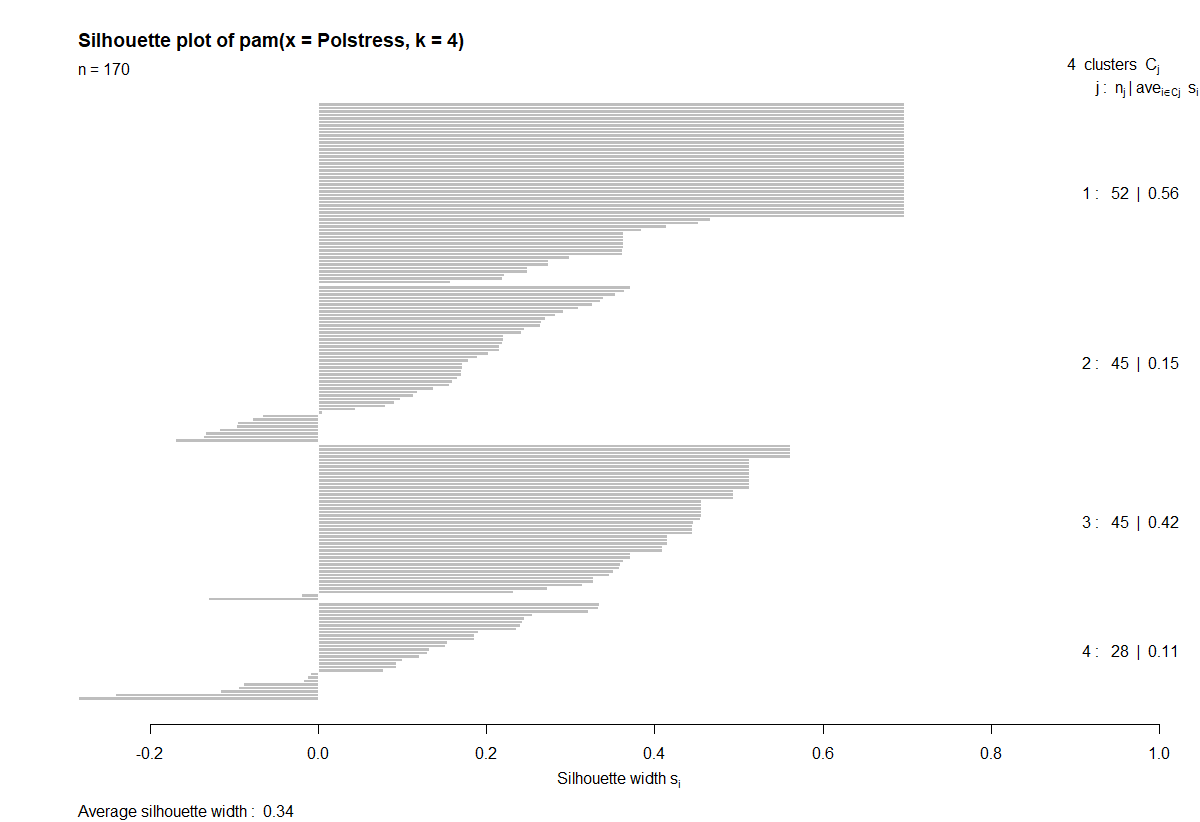
\includegraphics[width=8cm]{../../Graphs/Polstress-silhou.png}
\end{center}
\end{frame}
%%%%%%%%%%%%%%%%%%%%%%%%%
\section{Interpretation}
%%%%%%%%%%%%%%%%%%%%%%%
\begin{frame}
\frametitle{Interpretation}
What are the features behind a clusters: what feature/combination of features makes that an individual belong to a cluster.\\
\vspace{0.3cm}
A usual method consists of representing each feature against the clusters.
\end{frame}
%%%%%%%%%%%%%%%%%%%%%%%
\begin{frame}
\frametitle{Example}
{\bf Example}: 170 Swiss policemen recorded their emotional state in time using a questionnaire with ordinal scales (1 to 6). The features are 
\begin{itemize}
\item mood, 
\item stress, 
\item emotion, 
\item pressure, 
\item social support, 
\item situation familiarity, 
\item material support.
\end{itemize}
There is nothing to predict: the interest is to discover patterns in the data. 
\end{frame}
%%%%%%%%%%%%%%%%%%%%%%%%%%%%%
\begin{frame}
\frametitle{Example}
Below the scatter plots of the features (jittering points for more readability).
\begin{figure}[!h]
\centerline{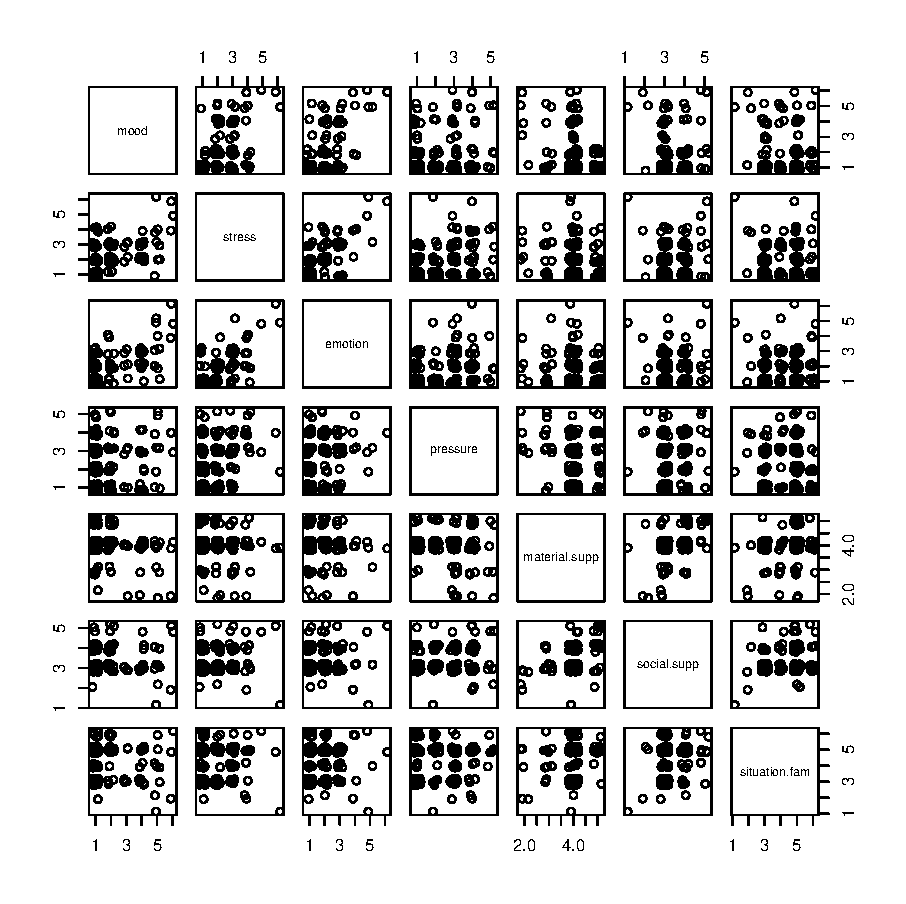
\includegraphics[width=7cm]{../../Graphs/Polstress-scat-jit.pdf}}
\end{figure}
\end{frame}
%%%%%%%%%%%%%%%%%%%%%%%%%%%%%%%
\begin{frame}
\frametitle{Example}
4 clusters of policemen were formed using AGNES. They can be analyzed by the feature values within each cluster. 
 \vspace{-1cm}
 \begin{figure}[!h]
 \centerline{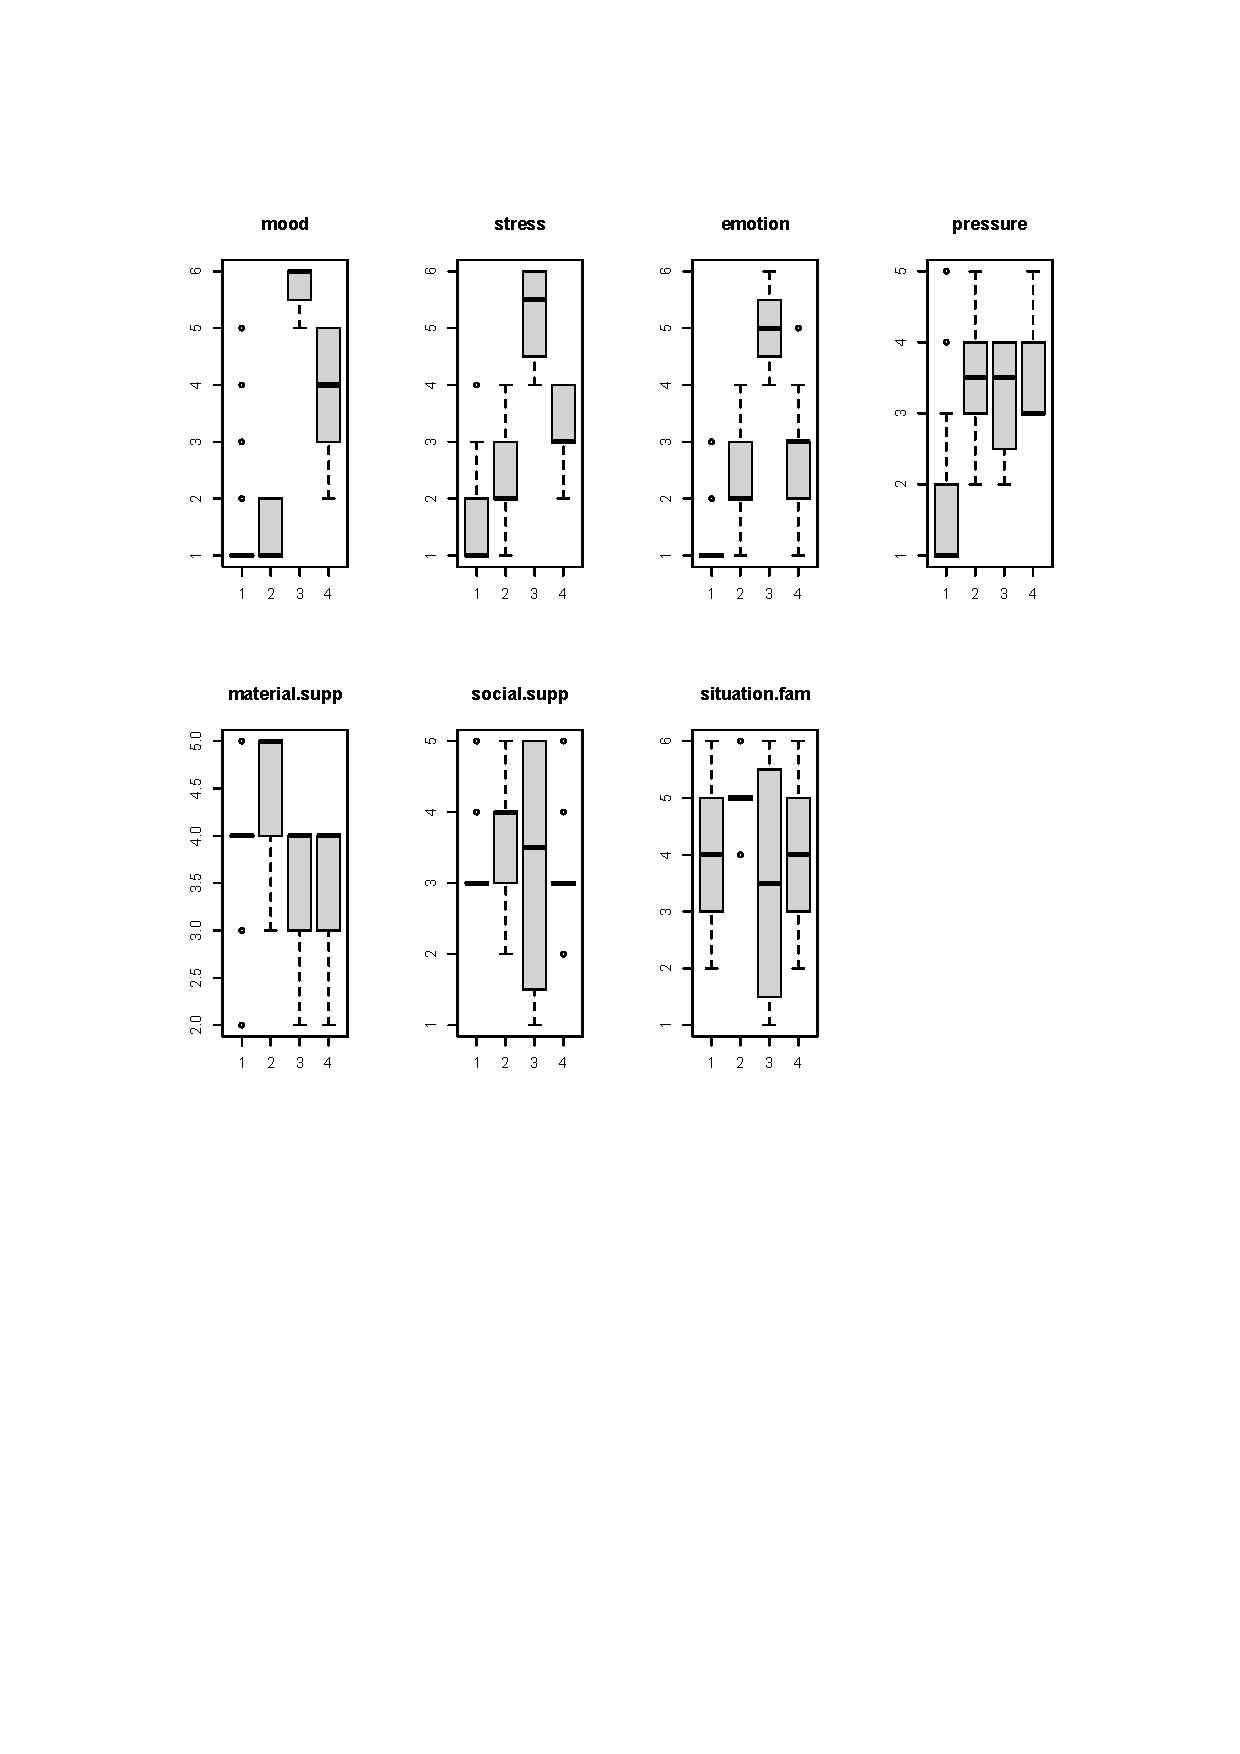
\includegraphics[width=9cm, height=11.5cm]{../../Graphs/Polstress-groups-4.pdf}}
  \end{figure}
\end{frame}
%%%%%%%%%%%%%%%%%%%%%%%%%%%%%%%
\begin{frame}
\frametitle{Example}
Some possible conclusions are
\begin{itemize}
\item Policemen in Cluster 3 have large mood, stress, and emotion values. 
\item Pressure characterizes cluster 1 (low) versus clusters 2 to 4 (medium).
\item Mood and stress are associated because clusters 1 to 4 have the same levels of these two features.
\end{itemize}
\end{frame}
%%%%%%%%%%%%%%%%%%%%%%%%%%%%%
\end{document}

\begin{frame}
\frametitle{Silhouette}
The {\bf silhouette} measures how "well" is an instance within its cluster. \\
\vspace{0.3cm}
Consider an instance $x$ assigned to cluster $C$. Let $d(x,A)$ be the distance from $x$ to any cluster $A$: the average dissimilarity between $x$ and all the instances in cluster $A$:
$$
d(x,A) = \frac{1}{|A|} \sum_{y\in A} d_{xy}.
$$ 
In particular, $d(x, C)$ is the distance from $x$ to its cluster. It measures how well $x$ is {\it integrated} to its cluster $C$.\\
\vspace{0.3cm}
A small $d(x,C)$ indicates a good clustering of $x$ within its cluster.
\end{frame}
%%%%%%%%%%%%%%%%%%%%%%%
\begin{frame}
\frametitle{Silhouette}
Now, consider the smallest average dissimilarities from $x$ to all the clusters to which it is not assigned:
$$
d(x,\bar{C}) = \min_{A\neq C} d(x, A) 
$$
This measures how $x$ is {\it separated} from the other clusters.\\
\vspace{0.3cm} 
A large $d(x,\bar{C})$ indicates a good separation of $x$ from all the other clusters (i.e. the one in which $x$ is not).
\end{frame}
%%%%%%%%%%%%%%%%%%%%%%%%%
\begin{frame}
\frametitle{Silhouette}
The silhouette of $x$ combines how well $x$ is integrated to its cluster and how well $x$ is separated from the other clusters:
$$
s_x=\frac{d(x,\bar{C})-d(x,C)}{\max\left\{d(x,\bar{C}),d(x,C)\right\}}
$$
The denominator ensures that $-1\leq s_x\leq 1$. The larger $s_x$, the better the clustering of $x$.\\
\vspace{0.3cm}
The average silhouette of all instances is taken as a measure of {\it goodness} of the clustering:
$$
s = \frac{1}{n}\sum_{i=1}^n s_{x_i}.
$$
The average silhouette should not be interpreted for itself. It is used to compare different clustering in order to choose $k$.
\end{frame}
%%%%%%%%%%%%%%%%%%%%%%%%%
\begin{frame}
\frametitle{Silhouette plot}
The {\bf silhouette plot} shows 
\begin{itemize}
\item the silhouettes of all the instances for a given PAM.
\item the average silhouette as an overall measure of goodness of clustering for this PAM. 
\end{itemize}
Next slides: cluster 1 and 3 are well formed (homogeneous and separated from the two other clusters), cluster 2 and 3 are less homogeneous. The average silhouette is 0.34. 
\end{frame}
%%%%%%%%%%%%%%%%%%%%%%%%%
\begin{frame}
\frametitle{Silhouette plot}
Policemen - PAM $k=4$ 
\begin{center}
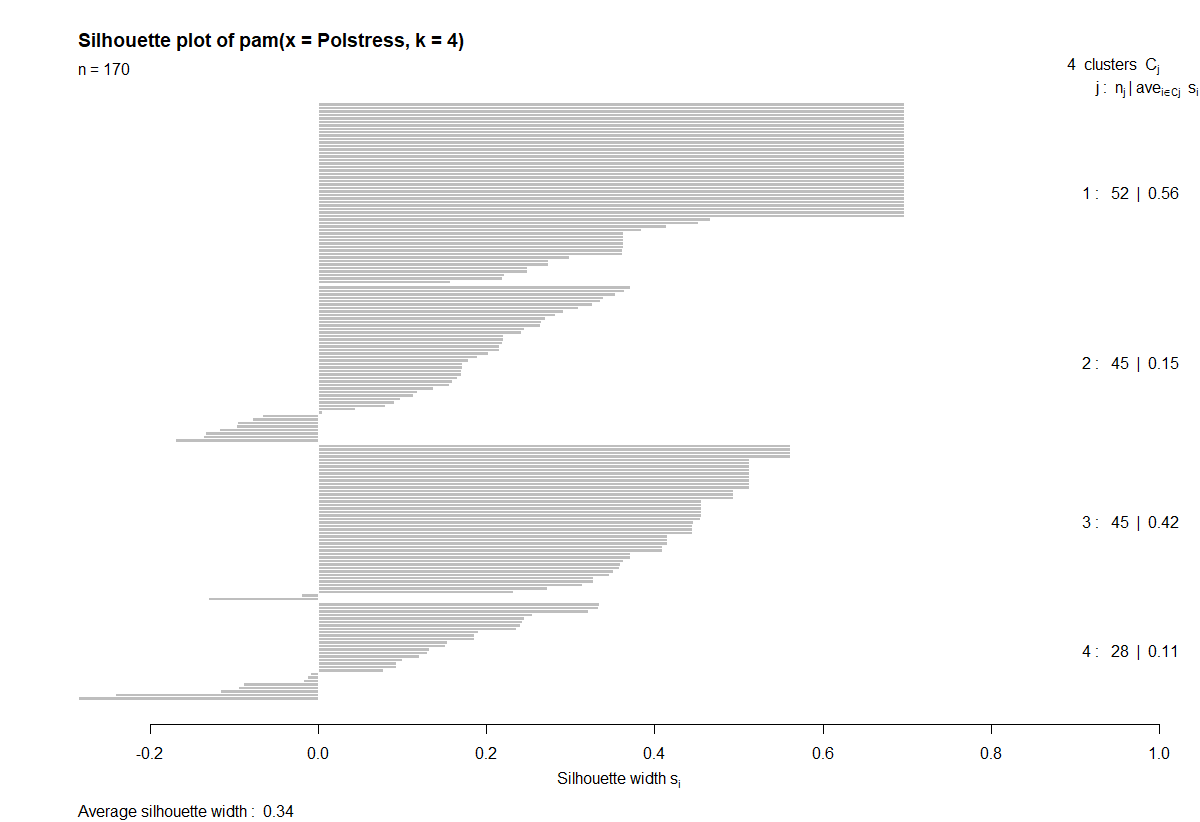
\includegraphics[width=8cm]{../../Graphs/Polstress-silhou.png}
\end{center}
\end{frame}
%%%%%%%%%%%%%%%%%%%%%%%%%
\begin{frame}
\frametitle{Example}
PAM on Policemen data (silhouettes):
\begin{center}
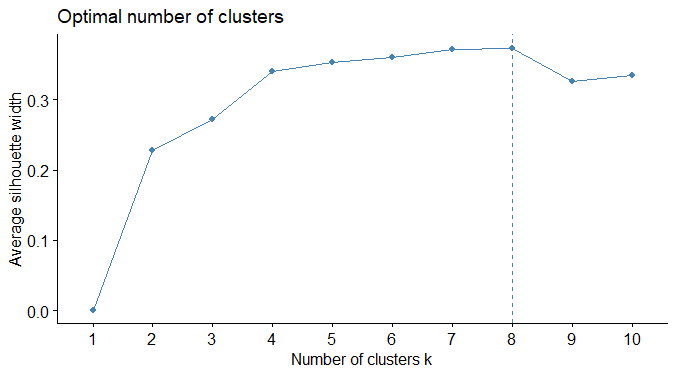
\includegraphics[width=8cm]{../../Graphs/Nb_pam_sil.png}
\end{center}
$k=8$ is a good choice here.
\end{frame}
%%%%%%%%%%%%%%%%%%%%%%%%%
\begin{frame}
\frametitle{Remarks}
\begin{itemize}
\item Hierarchical methods do not necessarily provide the best grouping since they are not reversible.
\item The method for computing the dissimilarity between clusters can also play an important role.
\item Extreme observations can have an important effect on the clustering result.
\end{itemize}
\end{frame}
%%%%%%%%%%%%%%%%%%%%%%%%%%%%%
\begin{frame}
\frametitle{Clustering}
The questions now are:
\begin{itemize}
\item How do we groups the policemen into 4 clusters?
\item How do we choose that 4 clusters is a ``good'' number?
\end{itemize}
Any clustering method is based on the definition of {\bf dissimilarities} (or similarities...). These are the same as for K-NN.
\end{frame}
%%%%%%%%%%%%%%%%%%%%%%%%%%%%%
%%%%%%%%%%%%%%%%%%%%%%%%%%%%%
%%%%%%%%%%%%%%%%%%%%%%%%%%%%%

%%%%%%%%%%%%%%%%%%%%%%%%%%%%%
\end{document}


\begin{frame}
\frametitle{Example}
K-means on Policemen data (silhouettes):
\begin{center}
\includegraphics[width=8cm]{../../Graphs/Nb_km_sil.png}
\end{center}
$k=8$ is a good choice here.
\end{frame}
%%%%%%%%%%%%%%%%%%%%%%%%%%%%%
\begin{frame}
\frametitle{Dissimilarities}
Any clustering method is based on the definition of {\bf dissimilarities} (or similarities...). These are the same as for K-NN.
\begin{itemize}
\item Most common for numerical features: Minkowski's (general $q$), Euclidean ($q=2$), Manhattan ($q=1$).
\item Most common for categorical features: Hamming distance.
\item Most common for mixed features: use dummy variables for categorical features and use a numerical distance.
\end{itemize}
Feature can (should?) be scaled.
\end{frame}
%%%%%%%%%%%%%%%%%%%%%%%%%%%%%
\begin{frame}[fragile]
\frametitle{Categorical features}
For categorical features, the {\bf Hamming distance} between two instances counts the number of features that are different. It assigns $1$ when the two levels are different and $0$ otherwise.\\
\vspace{0.2cm}
{\bf Example}: colors were added to the iris data. Possible levels are "violet","pale\_blue", "mauve", "pink", "yellow". The three first flowers are\\
\scriptsize
\begin{verbatim}
 Sepal.Length Sepal.Width Petal.Length Petal.Width Species  Color
1          5.1         3.5          1.4         0.2  setosa  mauve
2          4.9         3.0          1.4         0.2  setosa violet
3          4.7         3.2          1.3         0.2  setosa violet
\end{verbatim}
\normalsize
For the color, their Hamming distances are\\
\scriptsize
\begin{center}
\begin{tabular}{c|ccc}
 & 1& 2& 3\\
\hline
1 &0 &1 &1\\
2& 1& 0& 0\\
3& 1& 0& 0
\end{tabular}
\end{center}
\normalsize
\end{frame}
%%%%%%%%%%%%%%%%%%%%%%%%%%%%%
\begin{frame}
\frametitle{Mixed features in practice}
Hamming distance and Gower index are often replaced in practice by a pragmatic approach:
\begin{itemize}
\item Scale the numerical variables
$$
x_{ij} \rightarrow \frac{x_{ij} - \min\{x_{j}\}}{\max\{x_j\} - \min\{x_j\}}
$$ 
where $\min\{x_j\}=\min_{i'} x_{i'j}$ and $\max\{x_j\}=\max_{i'} x_{i'j}$ are the minimum and maximum of the variable $x_j$ (column-wise).
\item transform the categorical variables into their dummy variables: create one new column per level of $x_j$ with $0/1$ indicators. 
\end{itemize} 
\end{frame}
%%%%%%%%%%%%%%%%%%%%%%%%%%%%%
\begin{frame}
\frametitle{Dendrogram}
In order to build clusters, one 
\begin{itemize}
\item Select the wanted number of clusters,
\item Find the corresponding height on the tree,
\item Cut the tree branches at the height and see the clustering.
\end{itemize}
Alternatively, one can fix the height and see how many clusters it gives.
\end{frame}
%%%%%%%%%%%%%%%%%%%%%%%%%%%%%%
\begin{frame}
\frametitle{Dendrogram}
Below, 4 clusters grouped at height (dissimilarity) of about 6.5.
\begin{center}
\includegraphics[width=8cm]{../../Graphs/PolicemenDend2.png}
\end{center}
\end{frame}
%%%%%%%%%%%%%%%%%%%%%%%%%%%%%
\begin{frame}
\frametitle{Dendrogram}
Policemen's stress: dendrogram with complete linkage.
\begin{center}
\includegraphics[width=7cm]{../../Graphs/Polstress-dendro.pdf}
\end{center}
\end{frame}
%%%%%%%%%%%%%%%%%%%%%%%%%%%%%%
\begin{frame}
\frametitle{Example}
Policemen data with Gap (dendrogram with complete linkage):
\begin{center}
\includegraphics[width=8cm]{../../Graphs/Nb_agnes_hc_gap.png}
\end{center}
Not very conclusive. The software choice starts from the left ($K=1$) and conclude there is no reason to split the cluster. It is a local maximum. 8 or 10 could also be used here. 
\end{frame}
%%%%%%%%%%%%%%%%%%%%%%%%%%%%%
